\documentclass{article}
\usepackage[margin=1in,footskip=0.25in]{geometry}
\usepackage{booktabs}
\usepackage{listings}
\usepackage{xcolor}
\usepackage{graphicx} 
\usepackage{float}
\usepackage{amsmath}
\usepackage{times}
\usepackage{multirow}
\usepackage{subcaption}
\title{BTB Implementation in C}
\author{Kevin Evans \\ {\small 11571810}}

\begin{document}
	\maketitle
	\subsection*{Introduction}
	The Branch Target Buffer (BTB) is a prediction technique used to decrease the branch penalty in pipelined computer processors. This method stores a cache table containing an index, branch program address/counter (PC), a target PC, and a 2-bit prediction. When a branch occurs, it uses the BTB to lookup the mapped target. If the target is in the table, it uses the prediction value to determine whether to jump
	
	With a five-stage pipeline and without a BTB implementation, a branch can create a stall lasting for one or more clock cycles. It is important to utilize the BTB to ideally reduce the stalls to zero. In a non-ideal program, the BTB can introduce stalls: when there is a BTB miss, and a branch is taken, it creates 1 stall. In the case of a BTB hit resulting in a misprediction, the prediction must be scrapped creating 1 stall. 
	\subsubsection*{Program design}
	This program implements a branch target buffer (BTB) in C. The program accepts a text file trace of a previously-ran program, containing the program addresses as it progresses. The program reads the file line-by-line and creates a BTB containing the current PC with the next PC. As the trace file progresses, the BTB is used and several statistics are calculated, shown in the next section below. This program implements two state machines, shown below in Figure \ref{fig:statemachinea}. The state machine determines the ``next'' state of the prediction attribute of each entry in the BTB table.

	\begin{figure}[h]
		\centering
		\begin{subfigure}{0.45\textwidth}
			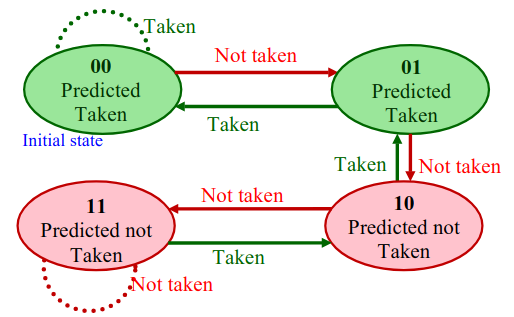
\includegraphics[width=\linewidth]{statemachineClass}
			\caption{}
			\label{subfig:class}
		\end{subfigure}
		\hfil
		\begin{subfigure}{0.45\linewidth}
			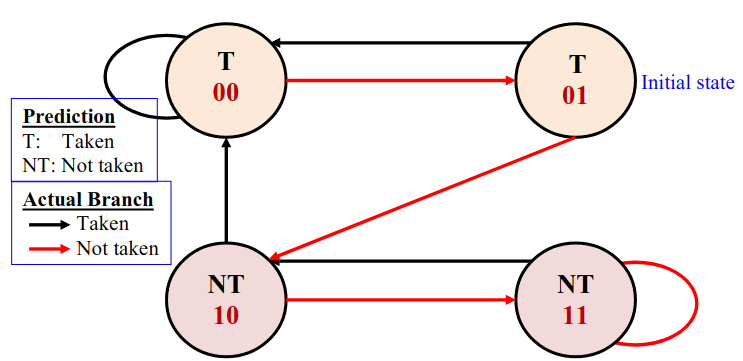
\includegraphics[width=\linewidth]{statemachineB}
			\caption{}
			\label{subfig:a}
		\end{subfigure}
		\caption{The two state machines used in this program, when determining the \textit{next} state of each BTB entry.}
		\label{fig:statemachinea}
	\end{figure}
	
	\pagebreak
	
	\subsection*{Parameters set and observed}
	Two benchmarks were used, \texttt{Li\_int} and \texttt{Dodoc\_FP}. These files contain traces of the execution of two programs, each with roughly 700K+ entries. The BTB is generated and we collect the hit/miss rate, number of correct/wrong entries, number of branches taken, BTB entry collisions, number of wrong addresses. We additionally calculate the number of additional stalls caused by the BTB misses and mispredictions, \begin{align}
		\text{approx. stalls} & = \text{IC} \times  \text{miss rate} \times \text{branch NT rate} \times 1 \text{ stall} \label{eq:stall} \\
			& \qquad + \text{IC} \times \text{hit rate} \times \text{misprediction rate} \times 1 \text{ stall}. \notag
	\end{align}
	
	\subsection*{Simulation results} 
	For both state machines and both benchmarks, the results are summarized in Table \ref{table:stats} and \ref{table:stats2}. These results are plotted in Fig. \ref{fig:graph}. Using \eqref{eq:stall}, the approximate stalls were calculated: $\approx 4000$ for \texttt{Li\_int}, $\approx 2000$ for \texttt{Dodoc\_FP}. Each of these is minuscule compared to the total number of branches causing a stall, $132694$ and $124254$ respectively.
		\begin{table}[p]
			\centering
			\caption{The results of two state machines using \texttt{Li\_int} trace.}
			\label{table:stats}
			$$\begin{array}{lcc}
				\toprule
				& \text{Class State Machine} & \text{State Machine B} \\
				\midrule
					\text{IC}                  & 716529  & 716529  \\
					\text{Hit}                 & 129557  & 129557  \\
					\text{Miss}                & 3137    & 3137    \\
					\text{Right}               & 109691  & 108999  \\
					\text{Wrong}               & 19866   & 20558   \\
					\text{Taken}               & 111571  & 111571  \\
					\text{Collision}           & 2535    & 2535    \\
					\text{Wrong addresses}         & 9954    & 9954    \\
					\text{Approx. stalls} & 4080 & 4205 \\
					\text{Total branches} & 132694 & 132694 \\
					\midrule
					\text{Hit rate}            & 97.64\% & 97.64\% \\
					\text{Prediction accuracy rate} & 84.67\% & 84.13\% \\
					\text{Incorrect address rate}   & 50.11\% & 48.42\% \\
					\text{Stall reduction} & 32.51\times & 31.55 \times \\
				\bottomrule
			\end{array}$$
		\end{table}
		\begin{table}[p]
			\caption{The results of two state machines using \texttt{Doduc\_FP} trace.}
			\label{table:stats2}
			$$\begin{array}{lcc}
				\toprule
				& \text{Class State Machine} & \text{State Machine B} \\
				\midrule
					\text{IC}                     & 724090  & 724090  \\
					\text{Hit}                    & 118421  & 118421  \\
					\text{Miss}                   & 5833    & 5833    \\
					\text{Right}                  & 111935  & 111786  \\
					\text{Wrong}                  & 6486    & 6635    \\
					\text{Taken}                  & 109320  & 109320  \\
					\text{Collision}              & 5114    & 5114    \\
					\text{Wrong addresses}        & 3576    & 3576    \\
					\text{Approx. stalls} & 1941 & 1965 \\
					\text{Total branches} & 124254 & 124254 \\
					\midrule
					\text{Hit rate}               & 95.31\% & 95.31\% \\
					\text{Prediction accuracy}    & 94.52\% & 94.40\% \\
					\text{Incorrect address rate} & 55.13\% & 53.90\% \\
					\text{Stall reduction} & 64.00 \times & 63.21 \times \\
				\bottomrule
			\end{array}$$
		\end{table}
	\begin{figure}[h]
		\centering
		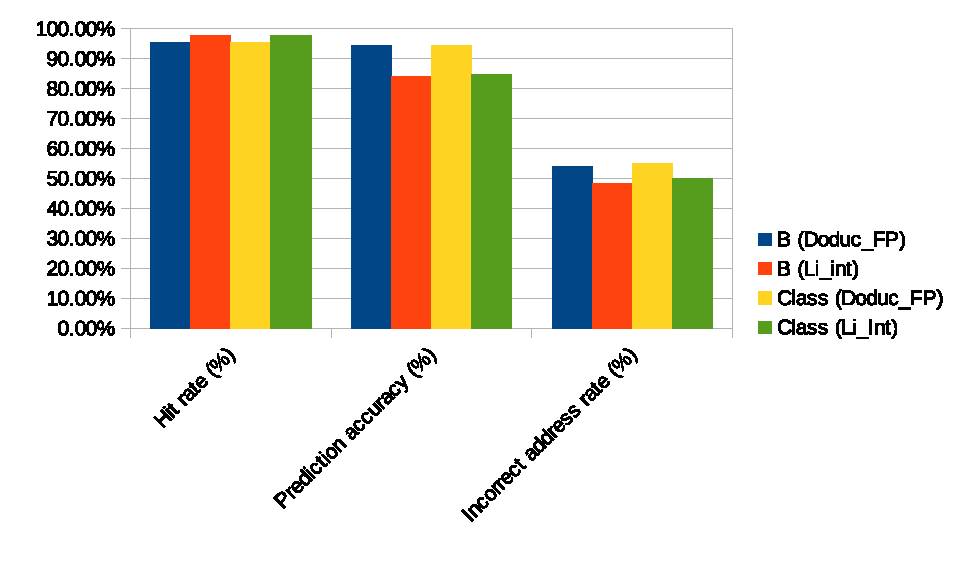
\includegraphics[width=0.7\linewidth]{grapheps}
		\caption{A comparison of the BTB results of the two state machines and two benchmarks.}
		\label{fig:graph}
	\end{figure}
	
	\subsection*{Quantitative assessment of results}
	Both state machines for both benchmarks performed well, achieving a prediction accuracy of roughly $84\%$ for both state machines in \texttt{Li\_int}; and a hit rate of $94\%$ for both machines in \texttt{Dodoc\_FP}. For these two benchmarks, using the BTB reduces the stalls and improves branch performance by 32 to 64 times. This was calculated using \begin{align}
		\text{\% stall reduction} & = \frac{\text{approx. stalls with BTB}}{\text{stalls without BTB}} = \frac{\text{approx. stalls with BTB}}{\text{total number of branches} \times 1 \text{ stall}}.
	\end{align}
	The significant reduction of stalls shows the importance of the 2-bit BTB on performance.
	
	\subsection*{Concluding remarks}
	This 2-bit BTB can greatly improve performance. The implementation of the 2-bit BTB in C achieved an accuracy rate exceeding 80\% and reduced the stalls by 32 to 64 times, for both state machines in two benchmarks. It would be advised to use branch prediction using a BTB on a pipelined processor, instead of not implementing a BTB. Other experiments could use a 1-bit or 3-bit predictor to potentially improve prediction accuracy.
	\pagebreak
	
	\subsection*{Appendix A: BTB simulation code}
	Please see the accompanying file \texttt{main.c}.
\end{document}